\section{Marco Teórico}
\label{ch:marcoTeorico}
% \subsection{Temas para el marco teórico}
% \label{sec:marco_teorico}
% \begin{itemize}
%     \item Organización y gestión de documentos electrónicos.
%     \item Arquitectura MVC.
%     \item Funcionamiento y características de los códigos QR.
%     \item Protocolo HTTPS y seguridad en las aplicaciones web.
%     \item Bases de datos relacionales.
%     \item Almacenamiento en la nube.
%     \item Usabilidad y experiencia de usuario (ux).
% \end{itemize}

\subsection{Organización y gestión de documentos electrónicos}
\label{sec:marco_teorico_tema1}
\subsubsection{Conceptos fundamentales}
La gestión documental electrónica es la gestión y organización de la información digital a lo largo de todo su ciclo de vida, su objetivo es garantizar la integridad, autenticidad, fiabilidad, disponibilidad y preservación de los documentos digitales a largo plazo.
El ciclo de vida de un documento digital se entiende como el conjunto de etapas de un documento desde su creación hasta su uso final, representado en la Figura \ref{fig:ciclo_vida}.

\begin{figure}[!tbh]
    \centering
    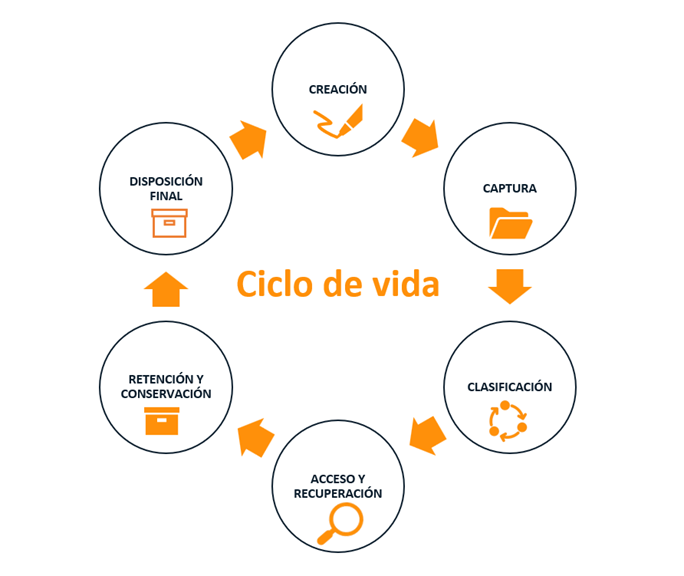
\includegraphics[width=0.6\linewidth]{img/ciclodevida.png}
    \caption{Diagrama del ciclo de vida de un documento digital \cite{imgCicloVida}}
    \label{fig:ciclo_vida}
\end{figure}

La organización de los documentos elctronicos es la clasificacion y gestion de los documentos de forma logica y normativa mediante sistemas tecnologicos, con la finalidad de poner a disposicion la información de forma más eficiente. 

En los sistemas de gestión documental actuales se utiliza el modelo llamado \textit{records continuum}, el cual ayuda a guiar la gestión documental electrónica, a diferencia de los modelos usados anteriormente, este modelo integra la administración de los documentos durante todo su ciclo de vida como un solo proceso continuo, administra el documento desde su creación, edición hasta su disposición final, esto asegura qué la información se mantenga segura y actualizada en los sistemas qué la almacenan.

\subsubsection{Impacto en la eficiencia institucional}
\cite{gestionDocGloriaAguirre} Expone la relación directa entre una gestión documental adecuada y el desempeño institucional, ya que con una gestión documental incorrecta hay perdidas de tiempo y dificultad en el acceso a la información, afectando directamente la eficiencia de la institución. Estos hallazgos destacan la necesidad de mejorar estos sistemas utilizando herramientas tecnológicas .

\subsection{Arquitectura Modelo-Vista-Controlador (MVC)}
\label{sec:marco_teorico_tema2}
\subsubsection{Definición y principios del patrón}
El propósito de los patrones de diseño es elevar la calidad del desarrollo de software, minimizando la redundancia y haciendo que los sistemas sean más fáciles de mantener. Entre ellos se encuentran los patrones arquitectónicos, cuya función es establecer la estructura fundamental de un sistema \cite{MVCFranklin}. 

La arquitectura MVC es un patrón de diseño que se centra en la ``separación de preocupaciones'', facilitando la gestión del código, la reutilización de componentes, y la escabilidad del sistema, además de que simplifica la repartición de tareas entre varias personas \cite{MVCpreprints}.

\subsubsection{Componentes y flujo de interacción}
La arquitectura MVC propone dividir la aplicación en tres módulos:
\begin{itemize}
    \item \textbf{Modelo:} Almacena representaciones abstractas de la información que el sistema va a procesar.
    \item \textbf{Vista:} Se encarga de mostrar la información a los usuarios mediante la interfaz.
    \item \textbf{Controlador:} Es el responsable de dirigir el flujo de la aplicación \cite{MVCFranklin}.
\end{itemize}

El flujo del sistema inicia cuando el usuario interactúa con la vista para ingresar datos o realizar solicitudes. Estas peticiones son recibidas y procesadas por el controlador, el cual se comunica con el modelo para manipular la información requerida y ejecutar la operación. Una vez concluido este procedimiento, el controlador notifica a la vista para que esta se actualice y presente los resultados finales al usuario. En la Figura \ref{fig:mvc_arquitectura} se ilustra este flujo de interacción entre los componentes.

\begin{figure}[!tbh]
    \centering
    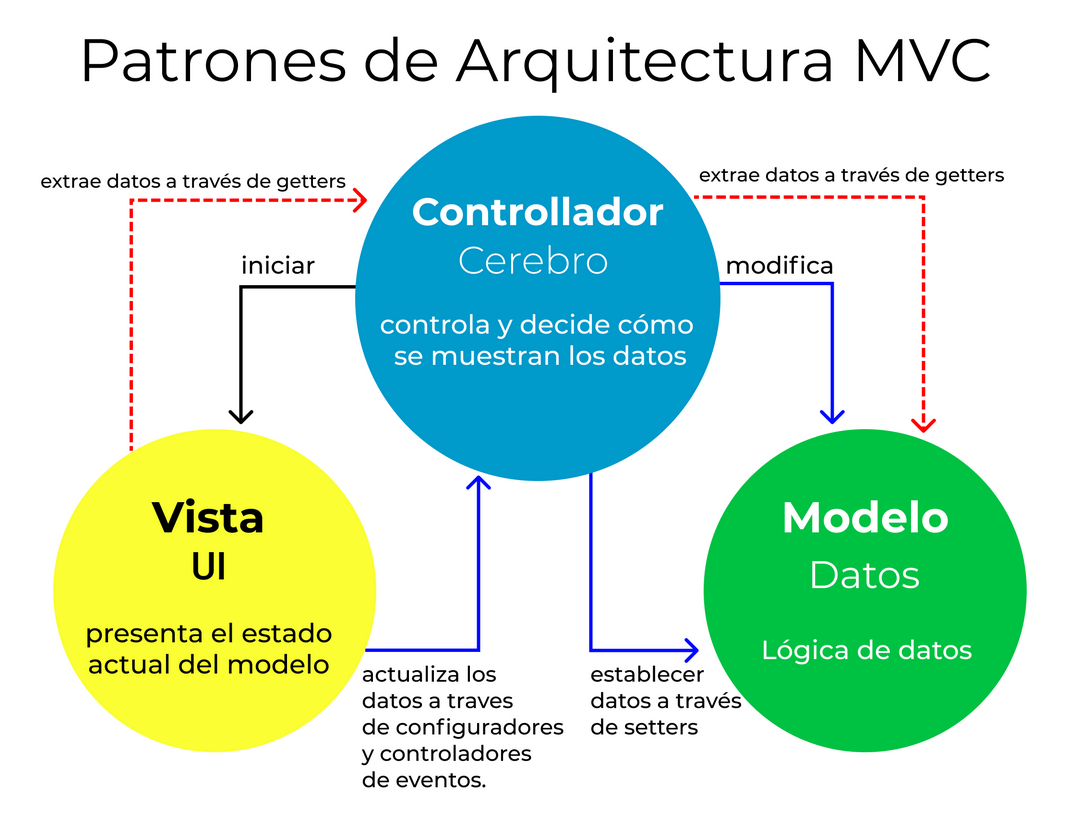
\includegraphics[width=0.7\linewidth]{img/arquitecturaMVC.png}
    \caption{Representación de la arquitectura MVC \cite{MVCfreecodecamp}}
    \label{fig:mvc_arquitectura}
\end{figure}

% \subsubsection{Justificación de uso en el proyecto}
% Este patrón arquitectónico resulta adecuado para este proyecto, ya que la lógica de negocio relacionada con la gestión documental, la generación de códigos QR y la presentación de interfaces deben mantenerse independientes para facilitar su mantenimiento y evolución. El análisis de la adopción de MVC en sectores como el empresarial y financiero subraya su amplia aceptación, aprovechándose para lograr una gestión superior de datos y una mejora en la experiencia del usuario \cite{MVCfreecodecamp}.

\subsection{Funcionamiento y características de los códigos QR}
\label{sec:marco_teorico_tema3}
Los códigos QR, códigos de respuesta rápida (Quick Response), son códigos de barras bidimensionales estructurados de forma matricial que permiten almacenar y recuperar información, al escanearlos con una cámara redirige a los usuarios a sitios web.

\subsubsection{Arquitectura física y estructura matricial}
\label{subsec:arquitectura_qr}
Un código QR distribuye la información tanto de forma horizontal como vertical dentro de una matriz cuadrada compuesta por módulos (puntos negros y blancos). La norma ISO/IEC 18004, la cual define las características de simbología y algoritmos de decodificación de los códigos QR, define un total de 40 versiones de códigos QR estándar, que van desde la Versión 1 (una matriz de 21x21 módulos) hasta la Versión 40 (177x177 módulos), incrementando la capacidad de almacenamiento de datos de forma proporcional al tamaño de la matriz \cite{QRISO18004}.

Para que las cámaras puedan interpretar la información, los códigos QR tienen componentes estructurales específicos y obligatorios como se muestra en la Figura \ref{fig:componentes_qr}:
\begin{itemize}
    \item Patrones de posición/búsqueda (Finder Patterns): Son los tres cuadrados grandes ubicados en las esquinas superiores e inferior izquierda. Su función es permitirle al software lector detectar la presencia del código, calcular su orientación exacta y determinar su tamaño, sin importar si el código se escanea de forma invertida o inclinada.
    \item Patrones de alineación y sincronización: Actúan como guías de referencia que ayudan al lector a corregir las distorsiones ópticas que ocurren cuando el código se captura desde ángulos desfavorables o sobre superficies con texturas.
    \item Zona silenciosa (Quiet Zone): Consiste en un margen blanco que debe rodear a todo el código para prevenir que elementos gráficos de alrededor, como el texto de la hoja del documento, interfieran con el proceso de lectura \cite{QRJeannot2024}.
\end{itemize}

\begin{figure}[!tbh]
    \centering
    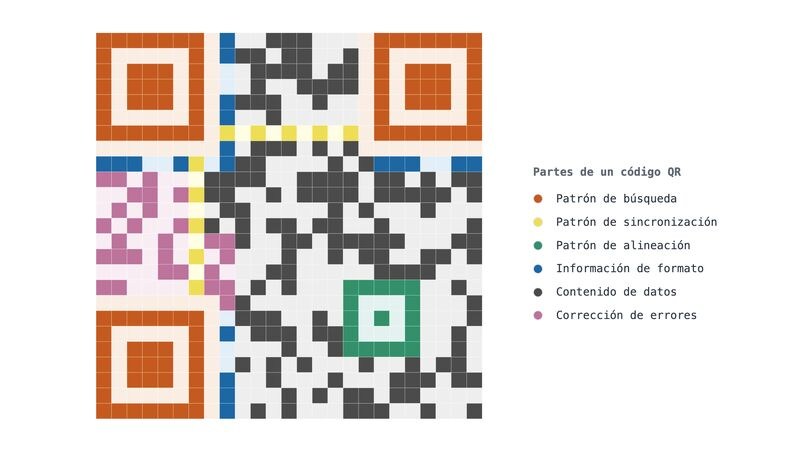
\includegraphics[width=0.7\linewidth]{img/QRcode.jpeg}
    \caption{Componentes principales de un código QR \cite{img_qr}}
    \label{fig:componentes_qr}
\end{figure}

\subsubsection{Mecanismo de decodificación y corrección de errores}
\label{subsec:mecanismo_qr}
Los códigos QR deben seguir siendo legibles aunque su impresión sufra daños, esto se logra mediante la integración del algoritmo de corrección de errores Reed-Solomon, el cual introduce redundancia matemática en los datos binarios durante la generación del código \cite{QRJeannot2024}. La norma ISO establece cuatro niveles de protección que puede tener el código QR: 

\begin{itemize}
    \item Nivel L (Low): Permite recuperar los datos si el código sufre hasta un 7\% de daño.
    \item Nivel M (Medium): Permite la recuperación con hasta un 15\% de daño.
    \item Nivel Q (Quarter): Soporta hasta un 25\% de daño o pérdida de superficie.
    \item Nivel H (High): Ofrece el máximo nivel, tolerando hasta un 30\% de destrucción.
\end{itemize}

%revision de ia
\subsection{Protocolo HTTPS y seguridad en las aplicaciones web}
\label{sec:marco_teorico_tema4}
El Protocolo Seguro de Transferencia de Hipertexto (HTTPS) es la forma segura del protocolo HTTP. Fue creado para proteger la autenticidad y confidencialidad de la información que viaja entre el navegador del usuario y el servidor web. Se basa en el protocolo de encriptación TLS (Seguridad de Capa de Transporte) para cifrar la comunicación en ambas direcciones en la capa de transporte \cite{diLuca2024hacking}.

Este protocolo se basa en un sistema de criptografia asimetrica, como se ilustra en la Figura \ref{fig:handshake_tls}, cuando un cliente intenta conectarse al servidor mediante una llave publica distribuida por medio de un certificado digital y una llave privada, empieza el proceso que se encarga de verificar la identidad del servidor y que genera una clave simetrica temporal, esa clave simetrica se usara para cifrar los datos durante esa sesion que es especifica, y asi se garantiza que el canal de comunicacion sera completamente ilegible para otros agentes externos.

\begin{figure}[!tbh]
    \centering
    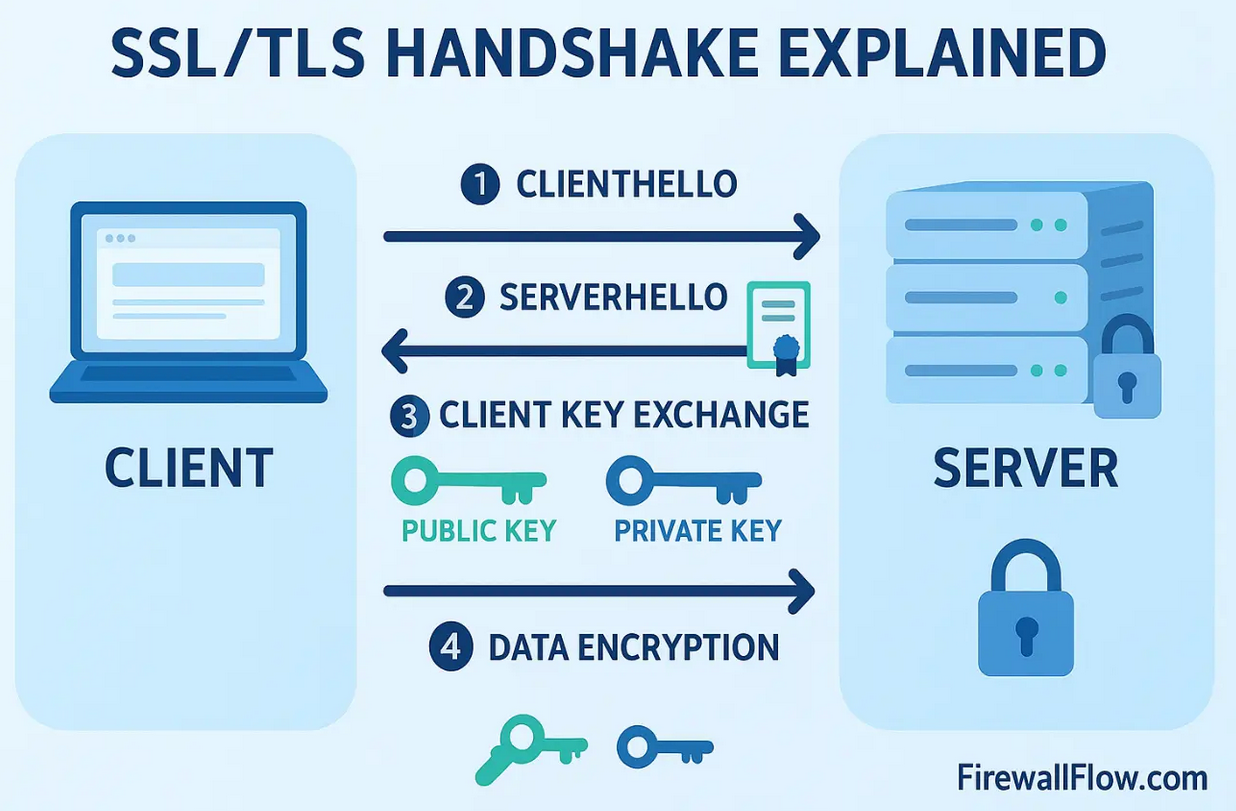
\includegraphics[width=0.6\linewidth]{img/handshake_tls.png}
    \caption{Proceso de establecimiento de conexión segura mediante SSL/TLS \cite{img_handshakeTLS}}
    \label{fig:handshake_tls}
\end{figure}

Al usar el protocolo HTTPS se garantiza que aunque haya un ataque que intercepte el trafico de red la información extraída no podra ser leida.

\subsubsection{Importancia en la gestión documental}
El uso del protocolo HTTPS es un requisito técnico obligatorio para todos los sistemas institucionales, ya que es indispensable  para proteger la información contra delitos como la divulgación de datos privados o el robo de información.
% Por el flujo de uso de este sistema es fundamental la seguridad en la capa de transporte, ya qué si se realizara el uso de este sistema por un canal sin cifrar, personas conectadas a la misma red podrían manipular el destino del usuario al escanear el código QR o impedir la visualización del documento. Con la implementación de HTTPS se asegura la protección de los documentos durante todo su ciclo de vida.

\subsection{Bases de datos relacionales}
\label{sec:marco_teorico_tema5}
El modelo relacional es el estándar para el diseño de bases de datos en aplicaciones de software a gran escala. Organiza la información en tablas bidimensionales compuestas por filas (registros) y columnas (atributos). Su principal ventaja es que permite representar vínculos y dependencias entre diferentes entidades del modelo de datos de forma intuitiva, ya que utiliza un sistema de claves primarias (\textit{Primary Keys}) y claves foráneas (\textit{Foreign Keys}) para establecer relaciones directas sin necesidad de crear jerarquías rígidas en el código de la aplicación. 

Este modelo garantiza la consistencia de los datos almacenados lo que es muy importante para sistemas qué manejan datos estructurados qué deben relacionarse de forma precisa con datos no estructurados \cite{camavilca2025inteligencia}.
\subsubsection{Integridad referencial y normalización}
Una característica de las bases de datos relaciones es que toda clave foránea en una tabla siempre debe corresponder siempre a una clave primaria válida en otra tabla, esto evita registros desvinculados y asegura el soporte transaccional, lo que garantiza qué los datos se guarden únicamente cuando no ocurren errores, lo qué disminuye la duplicación de datos y la inconsistencia en el almacenamiento. 

Las bases de datos de sistemas grandes suelen guardar y gestionar metadatos estructurales, comolos identificadores únicos, fechas de registro, o rutas hacia objetos en la nube, etc. por lo que se puede acceder a los datos de cada usuario y relacionarlos con sus acciones en el sistema \cite{camavilca2025inteligencia}. Estas características permite la conexión eficiente de los datos, lo que evita el aislamiento de la información y mejora la velocidad de consulta e interoperabilidad del sistema.

\subsection{Almacenamiento en la nube}
\label{sec:marco_teorico_tema6}
La nube es una red global de servidores qué almacenan y procesan datos de internet, esta tecnología permite el acceso de datos todo el tiempo y desde cualquier parte mediante el internet. Los servicios de almacenamiento en la nube sirven para guardar cantidades grandes de datos, y son utilizados en aplicaciones web o sistemas, ya qué ofrecen alta disponibilidad de los datos almacenados, y además tienen la capacidad de reducir o aumentar sus recursos conforme a su demanda y sin la necesidad de tener servidores físicos locales \cite{almaceamientoNube2024, aguilar2023caracteristicas}.

La Figura \ref{fig:nube_concepto}, ilustra las ventajas de la computación en la nube como la eliminación de la necesidad de mantener infraestructura física local y que todos los recursos pueden ser accesibles para cualquier persona mendiante internet.

\begin{figure}[!tbh]
    \centering
    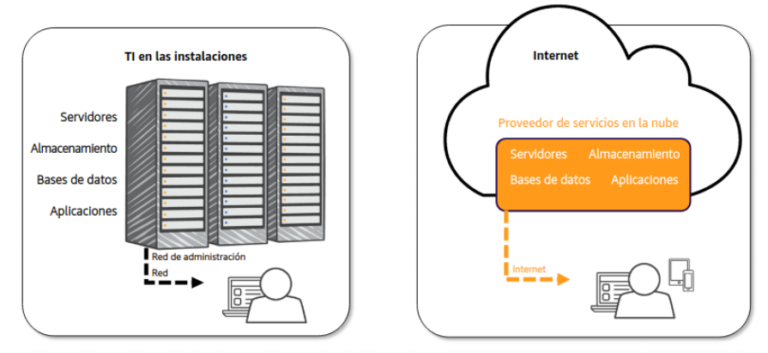
\includegraphics[width=0.8\linewidth]{img/nube_concepto.png}
    \caption{Comparativa entre infraestructura local y almacenamiento en la nube \cite{img_nube}}
    \label{fig:nube_concepto}
\end{figure}
\subsubsection{Uso en ámbitos corporativos y legales}
En las empresas del sector legal aún hay un gran uso de documentos físicos, lo qué hace más lento el proceso de digitalización de la información y desaprovecha las ventajas de las herramientas tecnológicas actuales \cite{NubeAmbitoLegal2025}. 

Para solucionar este problema la mejor solución es el almacenamiento en la nube, ya qué al implementarlo hay una reducción de costos operativos y optimización del uso de los archivos. Para lograr una adopción exitosa, los sistemas en la nube deben asegurar el cumplimiento normativo, reducir el riesgo de dependencia tecnológica de un proveedor específico y garantizar la seguridad de los datos digitalizados.

\subsection{Usabilidad y experiencia de usuario (UX)}
\label{sec:marco_teorico_tema7}
\subsubsection{Conceptos de Usabilidad y Experiencia de Usuario}
La usabilidad se enfoca en evaluar qué tan fácil, eficiente y libre de errores resulta para un usuario completar una tarea específica usando un producto. Mientras que la experiencia de usuario se enfoca en el nivel de satisfacción del usuario durante todo el tiempo que interactua con el producto, toma en cuenta las emociones y reacciones de la persona \cite{ferrer2023aplicabilidad}.

\subsubsection{Principios de evaluación e interacción}
Para garantizar la aceptación y uso adecuado de un sistema su diseño debe estar centrado en el usuario. La evaluación de la UX depende de criterios medibles del comportamiento del sistema, como la efectividad, la eficiencia y la curva de aprendizaje \cite{chihuahuaUX2024}. 

Una interfaz se considera exitosa cuando permite a los usuarios reconocer de forma intuitiva los patrones de navegación, logrando que el conocimiento adquirido al utilizar una función del sistema pueda aplicarse lógicamente en otras áreas. Asimismo, un sistema con un buen diseño evita esfuerzo del usuario, presenta la información de manera concisa y predictiva, asegurando que el software no genere nuevos problemas y cumpla con su finalidad correctamente \cite{chihuahuaUX2024}.

\subsubsection{Impacto en la adopción de sistemas de gestión documental}
En un sistema de gestión documental, la usabilidad y la experiencia de usuario son la conexión entre el entorno físico y el entorno digital. Si la interfaz web es confusa o difícil de utilizar, el usuario percibirá el sistema como una carga en lugar de una solución, lo que derivaría en resistencia al cambio y en el retorno al uso de documentos físicos, por lo que aplicar buenas prácticas de usabilidad es fundamental para asegurar el éxito de la digitalización de documentos \cite{ferrer2023aplicabilidad}.